\documentclass{article}
\usepackage[margin=1.5cm,bottom=2cm]{geometry}
\usepackage{fancyhdr}
\usepackage{graphicx}
\pagestyle{fancy}

\begin{document}
\fancyhead[L]{ 
\includegraphics[width=2cm]{au_logo.png} }
\fancyhead[R]{PHYS 2240: General Physics I}
\fancyfoot[C]{\thepage}
\vspace*{0cm}
\begin{center}
	{\LARGE \textbf{Quiz 6}}
	%\vspace{0.25cm}
	%{\Large Due: Friday, September 11}
\end{center}

On the surface of the Earth, a ball with radius $R$, mass $M$, and moment of inertia $I$ starts from rest at the top of a ramp of height $h$ and rolls to the bottom without slipping. If you ignore friction and air resistance, what is the speed of the ball at the bottom of the ramp, in terms of $m$, $g$, $h$, $R$, and $I$?
\begin{figure}[ht!]
	\centering
	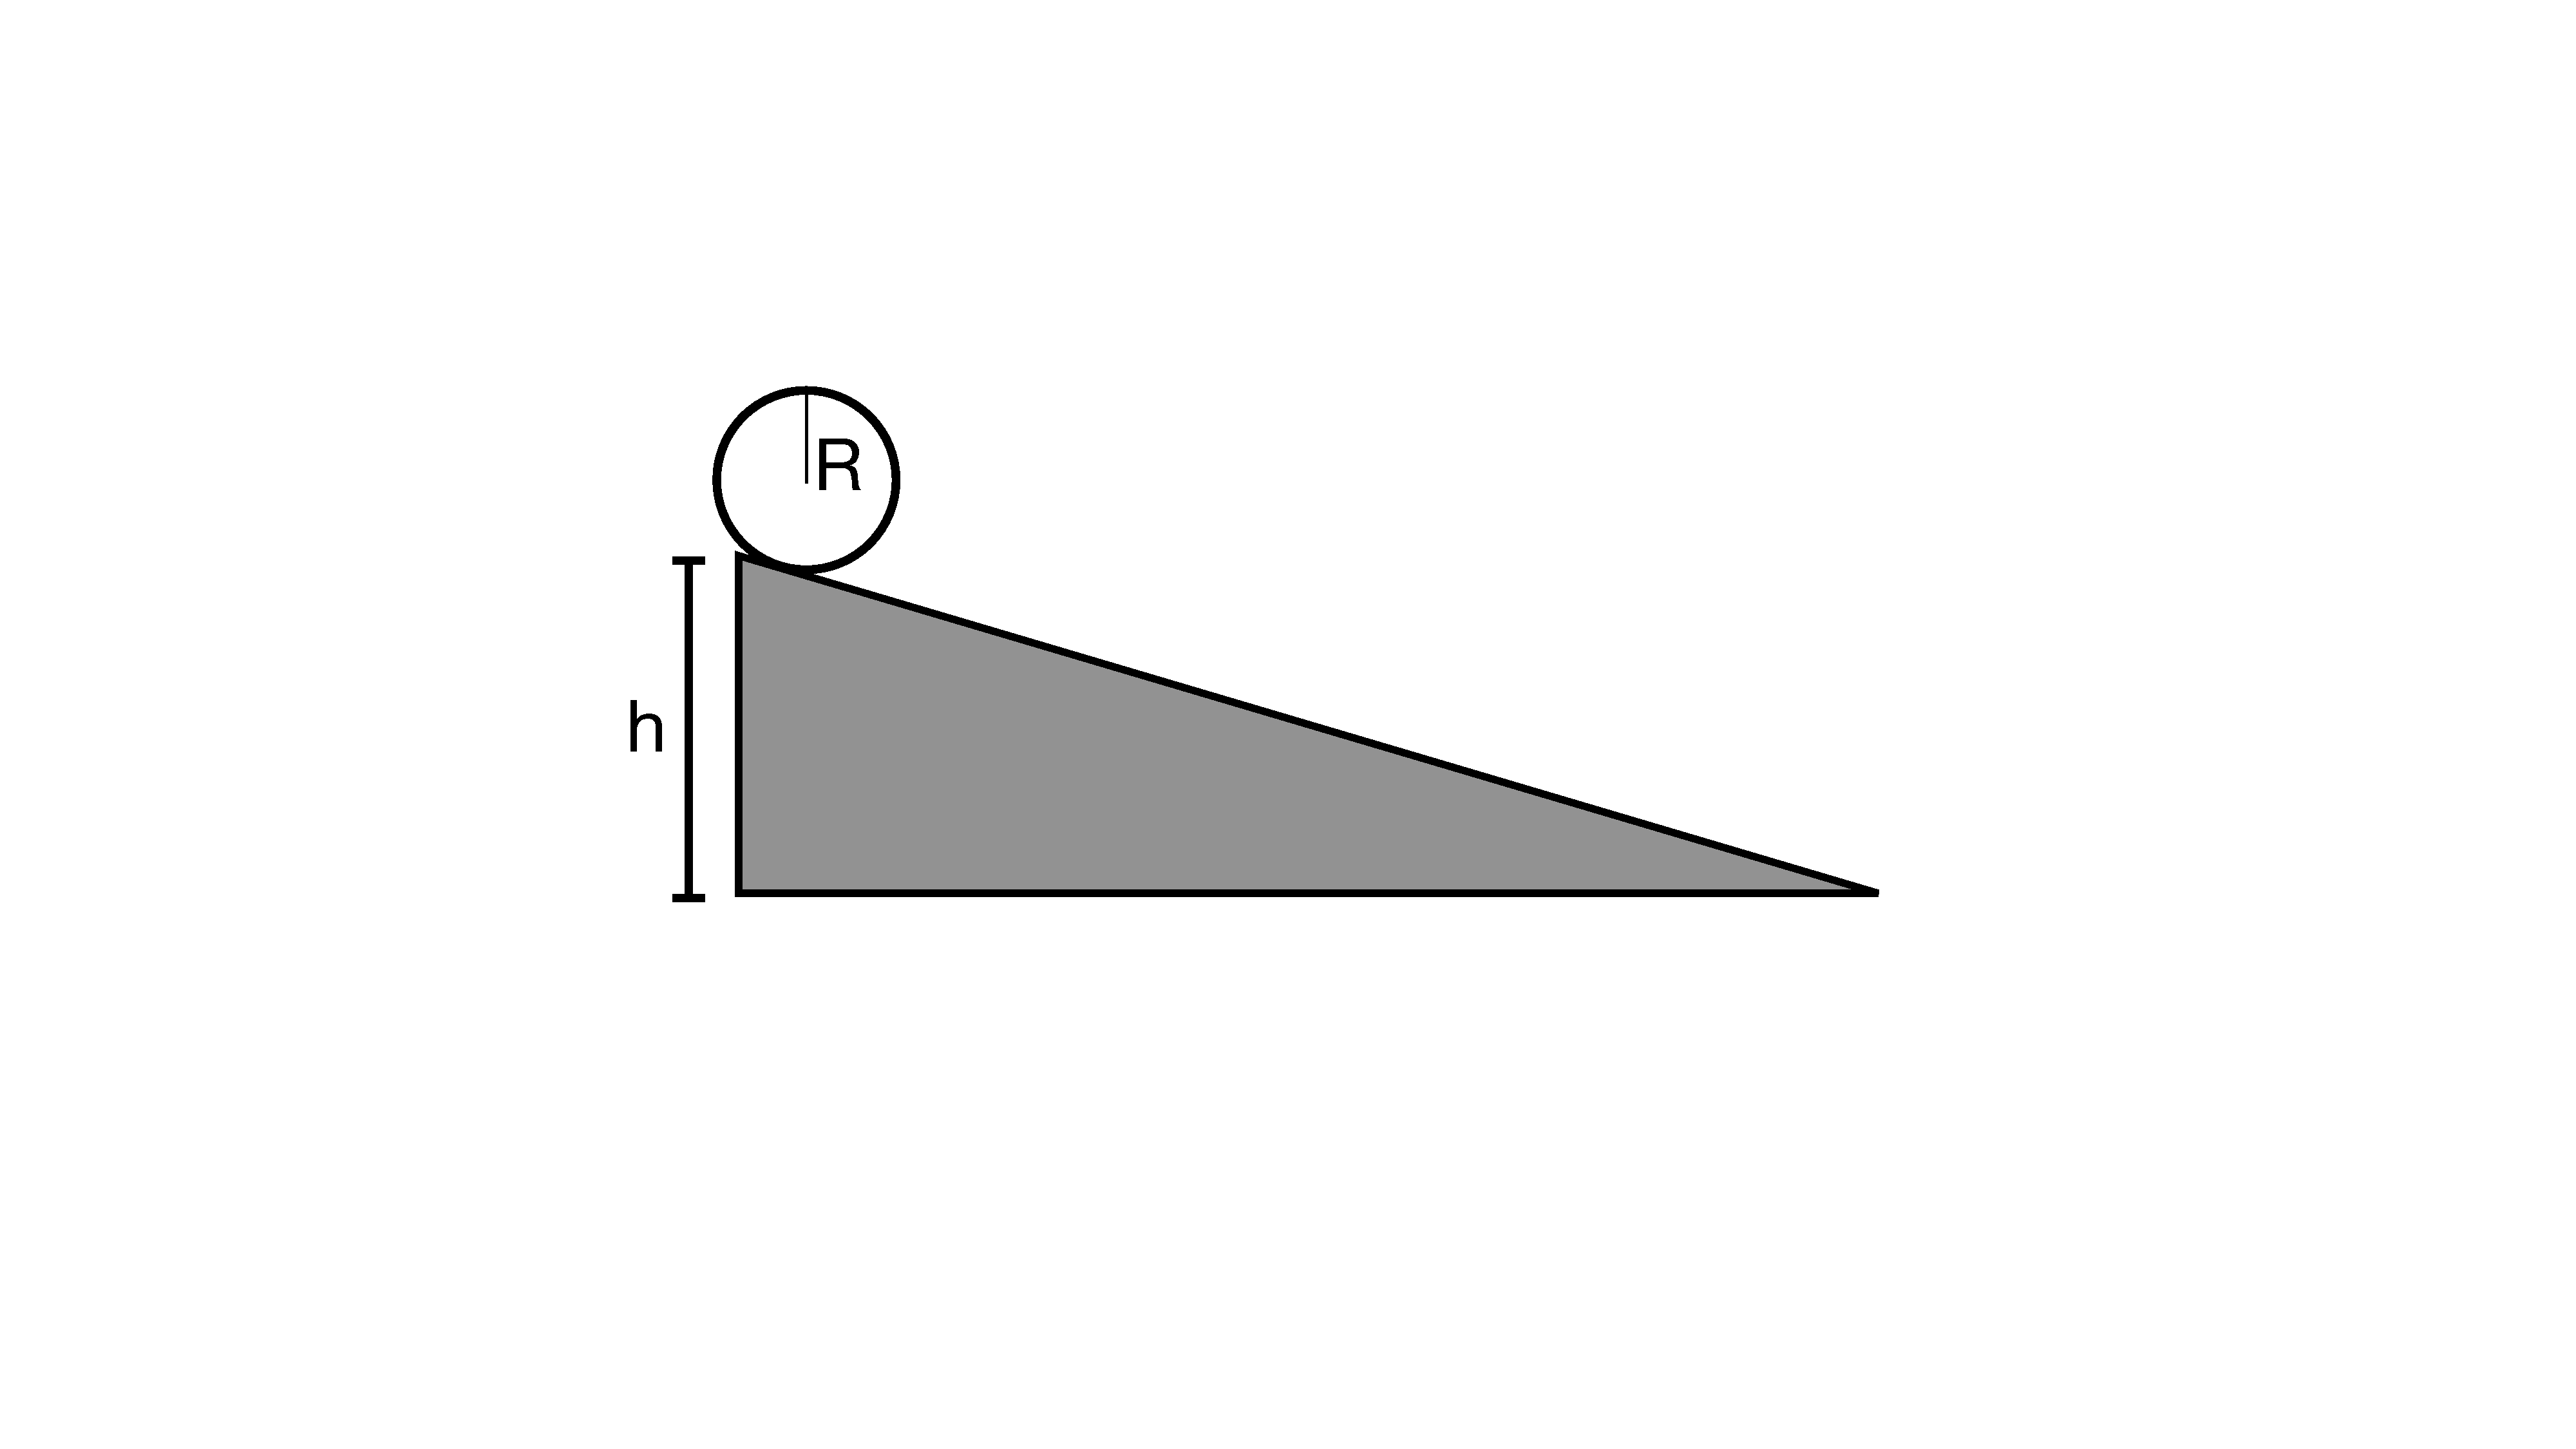
\includegraphics[width=6cm]{rolling_motion.pdf}
\end{figure}
\end{document}